% ================================================================= CHỈ SỐ LÂM SÀNG
\section{Chỉ số lâm sàng: hệ thống này dùng được đến đâu ở giường bệnh}
\label{sec:clinical}

F1 dò nhịp là chỉ số của người làm xử lý tín hiệu. Bác sĩ không quyết định gì dựa trên F1. Mục này đo
bốn đại lượng mà một máy theo dõi tim thai thật sự phải trả lời, trên \textbf{32 bản ghi, 269,6 phút tín
hiệu thật}: biến thiên ngắn hạn kiểu Dawes--Redman (STV), sai số nhịp tim thai theo Bland--Altman, độ phủ
theo \textbf{thời lượng}, và tần suất khoá nhầm nhịp mẹ. Mã tại \texttt{analysis/clinical.py}, số liệu
từng bản ghi tại \texttt{analysis/clinical\_results.json}.

\begin{canhbao}[title={Kết luận đặt ngay đầu mục, trước mọi con số}]
\textbf{Bộ dò này KHÔNG dùng được làm máy đo STV độc lập.} Trên tập con duy nhất đủ dài cho một trị số
Dawes--Redman hợp lệ (10 bản ghi Silesia B1, 20 phút mỗi bản), giới hạn đồng thuận 95\% là
$[-4{,}45;\ +8{,}14]$\,ms quanh một ranh giới quyết định mà hai mốc lâm sàng 2,6 và 3,0\,ms chỉ cách nhau
\textbf{0,4\,ms}. Ngay cả khi chỉ giữ những bản ghi mà cổng từ chối chấm ``cao'', bề rộng vẫn là 1,00\,ms
--- vẫn rộng gấp \textbf{2,5 lần} độ phân giải cần thiết. Nặng hơn: sai số \textbf{gần như chỉ đi một
chiều}, 25/32 bản ghi máy đọc STV \textbf{cao hơn} sự thật. Đó đúng là chiều \textbf{trấn an giả}.
\end{canhbao}

\subsection{Giao thức, khai báo trước khi chạy}

Epoch STV 3,75 giây (16 epoch/phút), trung bình khoảng RR trong epoch; STV là trung bình trị tuyệt đối
hiệu giữa hai epoch liên tiếp. RR hợp lệ 0,25--0,75\,s; epoch cần $\geq 2$ khoảng RR hợp lệ. Cửa sổ nhịp
tim thai 60 giây không chồng lấn (có quét thêm 5 / 10 / 30 giây). Dung sai khớp nhịp $\pm$50\,ms.

\begin{ghichu}[title={Một sai lệch có chủ ý so với kế hoạch, và lý do}]
Kế hoạch ban đầu dùng checkpoint \texttt{production\_22} cho 17 bản ghi Silesia. Nhưng
\texttt{production\_22} được huấn luyện \textbf{trên chính 17 chủ thể đó} --- đánh giá như vậy là trong
mẫu. Nhóm thay bằng checkpoint fold giữ lại đúng chủ thể, rồi chạy thêm \texttt{production\_22} chỉ để
\textbf{đo mức thổi phồng}: F1 trung bình 22 chủ thể là 97,51 (ngoài mẫu) so với 99,31 (trong mẫu), và
\textbf{độ chệch STV $+1{,}51$\,ms ngoài mẫu so với $+0{,}42$\,ms trong mẫu --- đánh giá trong mẫu làm
sai số STV nhỏ đi 3,6 lần}. Mọi con số trong mục này là ngoài mẫu.
\end{ghichu}

\subsection{Biến thiên ngắn hạn kiểu Dawes--Redman}

\begin{table}[H]\centering\small
\caption{STV nhãn so với STV mô hình. LoA là giới hạn đồng thuận Bland--Altman 95\%.}
\label{tab:stv}
\begin{tabular}{@{}L{3.6cm} C{0.8cm} C{1.8cm} C{1.8cm} C{1.7cm} C{2.8cm} C{1.6cm}@{}}
\toprule
\textbf{Tập} & $n$ & \textbf{STV nhãn} & \textbf{STV mô hình} & \textbf{Độ chệch} & \textbf{LoA 95\%} &
\textbf{Bề rộng} \\
\midrule
ADFECGDB & 5 & 9,62 & 9,95 & \tot{$+0{,}33$} & $[-0{,}89;\ +1{,}55]$ & 2,44 \\
Silesia B2 & 7 & 8,80 & 10,66 & $+1{,}86$ & $[-6{,}90;\ +10{,}63]$ & 17,53 \\
Silesia B1 & 10 & 7,74 & 9,59 & $+1{,}84$ & $[-4{,}45;\ +8{,}14]$ & 12,58 \\
CinC 2013 (PSD) & 10 & 5,54 & 26,04 & \xau{$+20{,}50$} & $[-24{,}76;\ +65{,}76]$ & 90,52 \\
\midrule
\textbf{Tất cả} & 32 & 7,58 & 15,02 & $+7{,}44$ & $[-23{,}05;\ +37{,}93]$ & 60,98 \\
\bottomrule
\end{tabular}
\end{table}

\begin{table}[H]\centering\small
\caption{Sai số STV bám rất sát chất lượng dò nhịp. Đơn vị ms.}
\label{tab:stv_f1}
\begin{tabular}{@{}L{4.0cm} C{0.9cm} C{2.0cm} C{2.2cm} C{2.2cm} C{2.4cm}@{}}
\toprule
\textbf{Dải F1} & $n$ & \textbf{Độ chệch} & \textbf{$|$sai số$|$ TB} & \textbf{$|$sai số$|$ max} &
\textbf{Bề rộng LoA} \\
\midrule
F1 $\geq 99{,}5$ & 18 & $+0{,}10$ & \tot{0,13} & 0,71 & \tot{0,92} \\
$99{,}0 \leq$ F1 $< 99{,}5$ & 2 & $+0{,}43$ & 0,43 & 0,46 & 0,19 \\
$95 \leq$ F1 $< 99$ & 3 & $+1{,}17$ & 1,17 & 1,61 & 2,12 \\
F1 $< 90$ & 9 & $+25{,}78$ & \xau{25,78} & \xau{67,14} & 79,48 \\
\bottomrule
\end{tabular}
\end{table}

Cơ chế rõ ràng và một chiều: mỗi dương tính giả hoặc âm tính giả làm nhiễu một khoảng RR, nhiễu đó cộng
vào hiệu giữa hai epoch liên tiếp, nên \textbf{mọi lỗi dò nhịp đều đẩy STV LÊN}. Sai số không ngẫu nhiên
--- nó luôn đi về phía ``biến thiên tốt, thai khoẻ''. Đo được: 25/32 bản ghi cao hơn nhãn, 7 bản thấp hơn
nhưng nhiều nhất chỉ $-0{,}17$\,ms.

\begin{table}[H]\centering\small
\caption{Bảng quyết định ở ngưỡng lâm sàng TRUFFLE.}
\label{tab:stv_nguong}
\begin{tabular}{@{}L{3.4cm} C{3.4cm} C{2.4cm} C{1.4cm} C{1.4cm} C{1.4cm}@{}}
\toprule
\textbf{Ngưỡng} & \textbf{Bản ghi nhãn dương} & \textbf{Máy gắn cờ} & \textbf{TP} & \textbf{FN} & \textbf{FP} \\
\midrule
STV $< 3{,}0$\,ms & 3 (a02, a07, a09) & 0 & \xau{0} & \xau{3} & 0 \\
STV $< 2{,}6$\,ms & 3 (a02, a07, a09) & 0 & \xau{0} & \xau{3} & 0 \\
\bottomrule
\end{tabular}
\end{table}

STV mô hình trên ba bản ghi đó là 21,81 / 42,57 / 67,63\,ms so với nhãn 1,18 / 0,93 / 0,49\,ms --- sai
một đến hai bậc độ lớn, luôn về phía trấn an.

\begin{canhbao}[title={Cảnh báo bắt buộc về ba bản ghi này}]
Chúng dài \textbf{60 giây}. Dawes--Redman cần tối thiểu 10 phút. Vì vậy 1,18 / 0,93 / 0,49\,ms
\textbf{không phải trị số STV lâm sàng hợp lệ}, và nhóm \textbf{không} tuyên bố đó là ba thai bị suy.
Nhóm đã kiểm tra: chuỗi RR nhãn không suy biến (a09 có 51 giá trị RR khác nhau, SD 16,1\,ms) --- trị số
thấp là do RR so le lên xuống. Điều bảng này chứng minh được chỉ là: \textbf{khi chuỗi tham chiếu nằm
trong dải thấp, mô hình không tái tạo được nó}.
\end{canhbao}

\begin{table}[H]\centering\small
\caption{Tập con hợp lệ nhất, và tại sao vẫn chưa đủ.}
\label{tab:stv_subset}
\begin{tabular}{@{}L{7.2cm} C{0.9cm} C{1.6cm} C{3.0cm} C{1.6cm}@{}}
\toprule
\textbf{Tập con} & $n$ & \textbf{Độ chệch} & \textbf{LoA 95\%} & \textbf{Bề rộng} \\
\midrule
Chỉ B1 --- 20 phút, tập duy nhất đủ dài cho Dawes--Redman & 10 & $+1{,}84$ &
$[-4{,}45;\ +8{,}14]$ & 12,58 \\
22 chủ thể trong miền & 22 & $+1{,}51$ & $[-4{,}88;\ +7{,}90]$ & 12,78 \\
\textbf{Cổng chấm CAO $+$ TRUNG BÌNH (= tất cả những gì máy thật sự trả lời)} & 23 & $+0{,}27$ &
$[-0{,}62;\ +1{,}16]$ & \textbf{1,78} \\
Chỉ cổng chấm CAO & 15 & $+0{,}11$ & $[-0{,}39;\ +0{,}61]$ & 1,00 \\
Tất cả 32 & 32 & $+7{,}44$ & $[-23{,}05;\ +37{,}93]$ & 60,98 \\
\bottomrule
\end{tabular}
\end{table}

Con số \textbf{có ý nghĩa vận hành} là hàng in đậm: sau khi cổng từ chối loại 9 bản ghi, LoA của những
gì máy trả lời là $[-0{,}62;\ +1{,}16]$\,ms, bề rộng 1,78\,ms. So với yêu cầu lâm sàng:

\begin{itemize}[leftmargin=1.5em,itemsep=2pt]
\item Phân biệt 2,6 với 3,0\,ms cần độ phân giải \textbf{0,4\,ms}. LoA 1,78\,ms rộng gấp \textbf{4,5 lần};
ngay cả 1,00\,ms của nhóm ``cao'' cũng gấp \textbf{2,5 lần}.
\item Bề rộng 1,78\,ms bằng \textbf{59\,\%} của chính ngưỡng 3,0\,ms, trên một thang mà bình thường là
5--9\,ms.
\item \textbf{Không một chủ thể nào trong 22 chủ thể trong miền có STV nhãn gần vùng bệnh lý} (thấp nhất
3,49\,ms ở B1\_05). Nghĩa là \textbf{chưa có một điểm dữ liệu hợp lệ nào trong vùng ra quyết định} ---
khẳng định ``mô hình phát hiện được STV thấp'' hiện \textbf{không kiểm chứng được}, chứ không phải
``đã bác bỏ''.
\end{itemize}

\begin{figure}[H]\centering
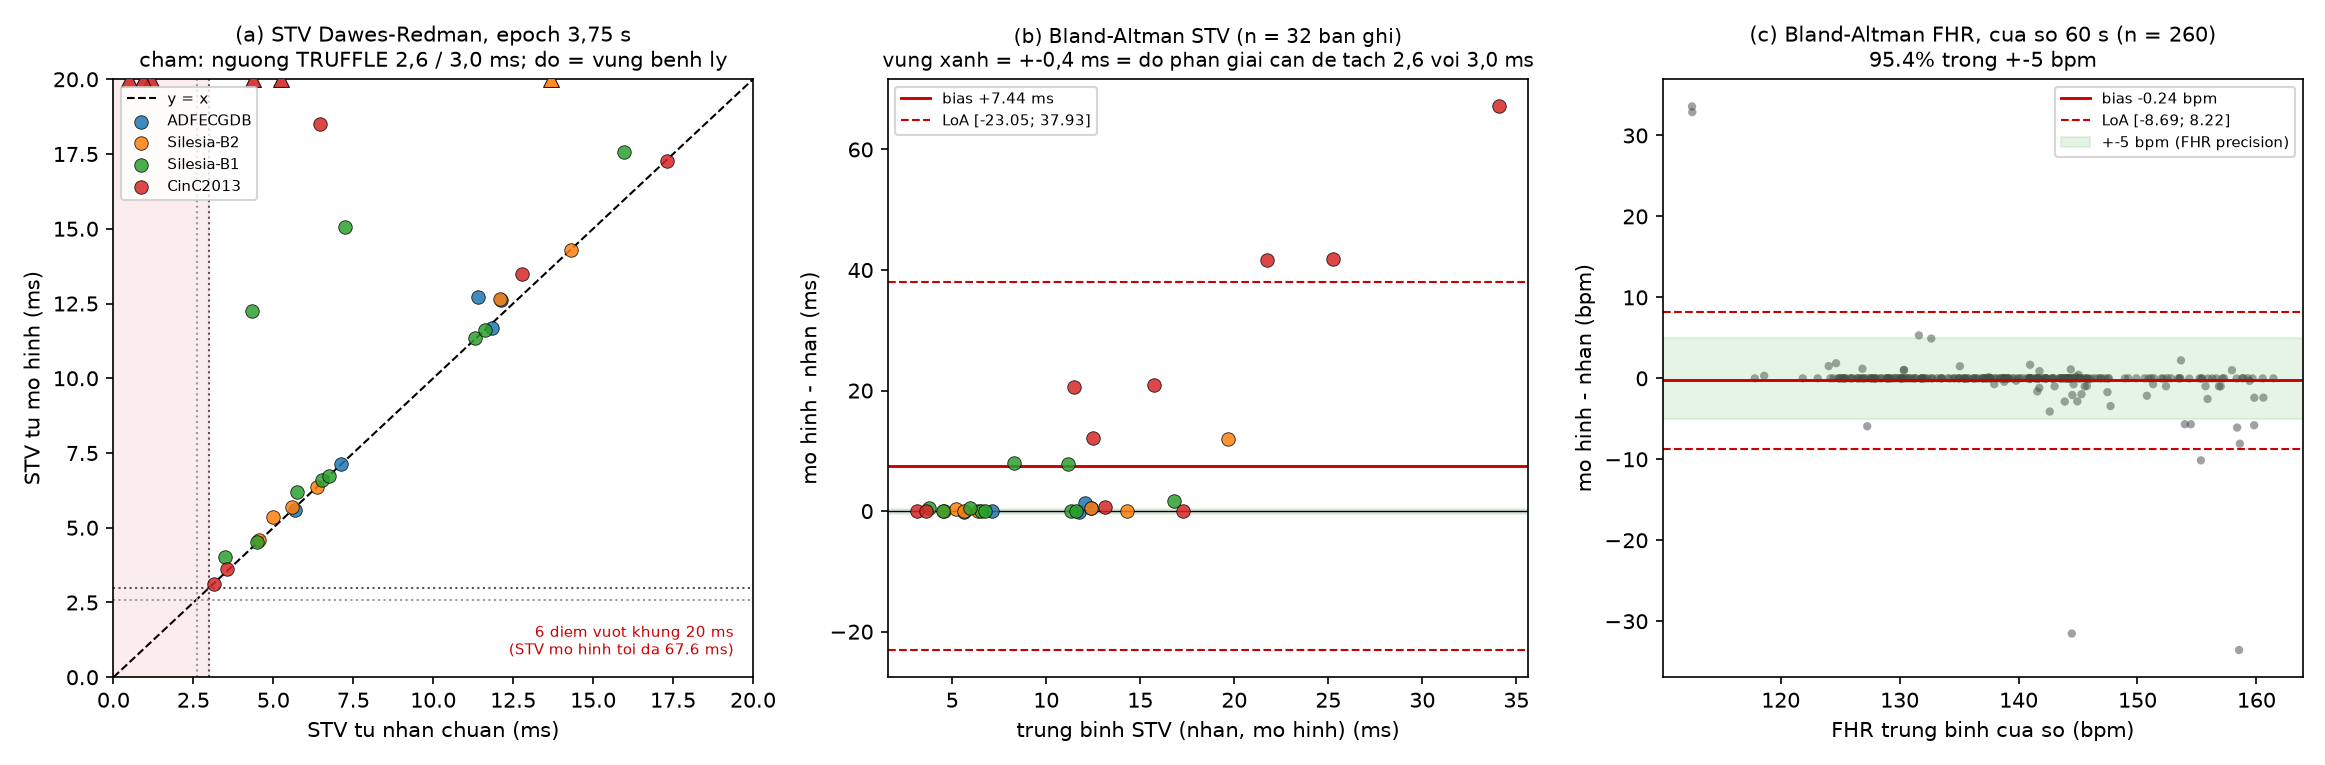
\includegraphics[width=\textwidth]{figs/clinical_stv_fhr.png}
\caption{(a) STV nhãn so với STV mô hình, phóng to vùng lâm sàng (vùng đỏ là bệnh lý). (b) Bland--Altman
cho STV. (c) Bland--Altman cho nhịp tim thai, cửa sổ 60 giây. Nguồn: \texttt{analysis/clinical.py}.}
\label{fig:clin_stv}
\end{figure}

\subsection{Nhịp tim thai --- đây là chỗ hệ thống thật sự dùng được}

\begin{table}[H]\centering\small
\caption{Bland--Altman nhịp tim thai, cửa sổ 1 phút. Mẫu số là số cửa sổ nhãn hợp lệ; 260/260 cửa sổ đều
ghép cặp được, không cửa sổ nào bị loại vì mô hình không tính nổi.}
\label{tab:fhr}
\begin{tabular}{@{}L{3.4cm} C{1.6cm} C{1.8cm} C{3.0cm} C{1.4cm} C{2.6cm}@{}}
\toprule
\textbf{Tập} & \textbf{$n$ cửa sổ} & \textbf{Độ chệch} & \textbf{LoA 95\%} & \textbf{MAE} &
\textbf{\% trong $\pm5$ bpm} \\
\midrule
ADFECGDB & 25 & $+0{,}11$ & $[-0{,}62;\ +0{,}83]$ & 0,14 & \tot{100,00} \\
Silesia B2 & 35 & $-0{,}41$ & $[-3{,}74;\ +2{,}91]$ & 0,61 & 91,43 \\
Silesia B1 & 190 & $+0{,}15$ & $[-6{,}88;\ +7{,}18]$ & 0,70 & 97,37 \\
CinC 2013 (PSD) & 10 & $-7{,}81$ & $[-34{,}60;\ +18{,}99]$ & 9,00 & \xau{60,00} \\
\midrule
\textbf{Tất cả} & 260 & $-0{,}24$ & $[-8{,}69;\ +8{,}22]$ & 0,95 & \textbf{95,38} \\
\bottomrule
\end{tabular}
\end{table}

Độ chệch ổn định ở $-0{,}23$\,bpm ở mọi độ dài cửa sổ: \textbf{không có sai lệch hệ thống về nhịp};
toàn bộ bề rộng LoA là do các bản ghi hỏng, không do sai số phân bố đều.

\begin{table}[H]\centering\small
\caption{Quét độ dài cửa sổ. Bài DPSS không nêu độ dài cửa sổ dùng cho ``FHR precision 88,61\,\%'';
cửa sổ càng dài càng dễ, nên nhóm quét cả dải. Giá trị là \% cửa sổ trong $\pm5$\,bpm.}
\label{tab:fhr_quet}
\begin{tabular}{@{}L{3.6cm} C{2.4cm} C{2.4cm} C{2.4cm} C{2.4cm}@{}}
\toprule
\textbf{Tập} & \textbf{5\,s} & \textbf{10\,s} & \textbf{30\,s} & \textbf{60\,s} \\
\midrule
ADFECGDB & \tot{98,66} ($n$=299) & \tot{98,66} ($n$=149) & 100,00 ($n$=50) & 100,00 ($n$=25) \\
Silesia B2 & 94,99 ($n$=419) & 94,26 ($n$=209) & 92,86 ($n$=70) & 91,43 ($n$=35) \\
Silesia B1 & 95,98 ($n$=2389) & 95,63 ($n$=1190) & 97,44 ($n$=390) & 97,37 ($n$=190) \\
CinC 2013 & 55,00 ($n$=120) & 51,67 ($n$=60) & 60,00 ($n$=20) & 60,00 ($n$=10) \\
\midrule
\textbf{Tất cả} & 94,58 ($n$=3227) & 94,09 ($n$=1608) & 95,66 ($n$=530) & 95,38 ($n$=260) \\
\bottomrule
\end{tabular}
\end{table}

Trên ADFECGDB, \textbf{ngay ở cửa sổ khắt khe nhất đã thử (5 giây) vẫn đạt 98,66\,\%}, cao hơn 88,61\,\%
của DPSS. Đây là so sánh \textbf{bảo vệ được}: không thể nói nhóm thắng nhờ chọn cửa sổ dài. Vẫn phải
kèm ba điều kiện: (i) DPSS chạy zero-shot từ FECGSYNDB tổng hợp còn đây là tách bản ghi trong miền ---
\textbf{hai giao thức khác nhau}; (ii) nhóm chưa chạy lại DPSS, đây là so với con số đã công bố;
(iii) $n = 5$ sản phụ.

\subsection{Độ phủ theo THỜI LƯỢNG, không theo bản ghi}

\begin{canhbao}[title={Một cách gọi tên sai phải sửa}]
Con số 43,8\,\% trong \texttt{facts\_phase2.json} và trong bản v3.2 là \textbf{tỉ lệ BẢN GHI được chấm
xanh}, \textbf{không} phải độ phủ thời gian. Hai đại lượng khác nhau và đang bị dùng lẫn. Từ đây mọi
tuyên bố về độ phủ đều là \textbf{\% thời lượng}.
\end{canhbao}

Ba chính sách khai báo trước: \textbf{P1} trả lời trừ đoạn đỏ; \textbf{P2} chỉ trả lời đoạn xanh;
\textbf{P3} như P1 nhưng bỏ cả bản ghi nếu độ tin cậy mức bản ghi là thấp.

\begin{table}[H]\centering\small
\caption{Độ phủ theo thời lượng và --- quan trọng hơn --- độ dài khoảng trống liên tục.}
\label{tab:phu}
\begin{tabular}{@{}L{2.8cm} C{1.6cm} C{1.5cm} C{1.3cm} C{1.3cm} C{1.7cm} C{3.4cm}@{}}
\toprule
\textbf{Tập} & \textbf{Thời lượng} & \textbf{Đoạn 4\,s} & \textbf{P1} & \textbf{P2} & \textbf{P3} &
\textbf{Khoảng trống P1: TV / p90 / max} \\
\midrule
ADFECGDB & 25,0 phút & 375 & \tot{96,0} & 88,8 & 96,0 & 4\,s / 12\,s / \textbf{12\,s} \\
Silesia B2 & 35,0 phút & 525 & 88,2 & 61,3 & 81,0 & 4\,s / 12\,s / \textbf{56\,s} \\
Silesia B1 & 199,6 phút & 2990 & 88,8 & 58,8 & 75,8 & 4\,s / 12\,s / \xau{192\,s} \\
CinC 2013 & 10,0 phút & 150 & \xau{58,7} & 42,7 & 39,3 & 8\,s / 33\,s / 48\,s \\
\midrule
\textbf{Tất cả} & \textbf{269,6 phút} & 4040 & \textbf{88,2} & 61,3 & 68,7 & 4\,s / 16\,s / \xau{192\,s} \\
\bottomrule
\end{tabular}
\end{table}

\begin{table}[H]\centering\small
\caption{Đối chiếu với chuẩn lâm sàng. \textbf{Các mốc CTG dưới đây do phản biện cung cấp và nhóm CHƯA
đối chiếu bản gốc} --- phải kiểm chứng trước khi đưa vào bài báo.}
\label{tab:phu_chuan}
\begin{tabular}{@{}L{5.4cm} C{2.6cm} L{6.4cm}@{}}
\toprule
\textbf{Chuẩn} & \textbf{Mất tín hiệu} & \textbf{\hethong{} tương ứng} \\
\midrule
CTG Doppler giai đoạn I & 5--8\,\% & ADFECGDB \tot{4,0\,\%} đạt; Silesia 11,2--11,8\,\% \xau{chưa đạt};
CinC 41,3\,\% \xau{chưa đạt} \\
CTG Doppler giai đoạn II & 9--20\,\% & Silesia nằm trong dải này \\
fECG bụng thương mại & 5,3\,\% & chỉ ADFECGDB đạt \\
``Mất tín hiệu cao'' & $> 20$\,\% & chỉ CinC vượt \\
\bottomrule
\end{tabular}
\end{table}

\begin{canhbao}[title={Tổng phần trăm không phải con số quan trọng nhất --- độ dài khoảng trống mới là}]
Trung vị khoảng trống là 4 giây (một đoạn đơn lẻ), vô hại. Đuôi phân bố mới là chỗ nguy hiểm:
\textbf{p90 $= 16$ giây, max $= 192$ giây} (B1\_07), và 48--64 giây ở B1\_06, B1\_10, B2\_03.

Nhịp giảm muộn kéo dài 30--90 giây; nhịp giảm kéo dài theo định nghĩa là 2--10 phút.
\textbf{Một khoảng trống 192 giây có thể giấu trọn một cơn giảm kéo dài mà máy không hề báo.}
Ở chính sách P2 (chỉ tin đoạn xanh) khoảng trống lớn nhất là \textbf{528 giây}, không thể chấp nhận
trên lâm sàng. Vì vậy mọi tuyên bố về độ phủ trong bài báo \textbf{bắt buộc} kèm p90 và max của khoảng
trống.
\end{canhbao}

Độ phủ chỉ 88,2\,\% \textbf{vì} cổng từ chối đang làm việc của nó. Nếu tắt cổng, máy trả lời 100\,\%
thời lượng nhưng 9/32 bản ghi sẽ trả kết quả sai (F1 từ 19,35 đến 89,45). Đây là một \textbf{đánh đổi}
và phải trình bày như đánh đổi, không được trình bày 88,2\,\% như khuyết điểm thuần tuý hay 100\,\%
như ưu điểm.

\begin{table}[H]\centering\small
\caption{Cổng từ chối có phân tầng đúng không.}
\label{tab:cong_tang}
\begin{tabular}{@{}L{2.8cm} C{0.9cm} C{1.6cm} C{1.6cm} C{2.4cm} C{2.4cm}@{}}
\toprule
\textbf{Mức cổng} & $n$ & \textbf{F1 TB} & \textbf{F1 min} & \textbf{$|\Delta$STV$|$ TB} &
\textbf{$|\Delta$STV$|$ max} \\
\midrule
cao & 15 & 99,92 & 99,61 & 0,15\,ms & 0,71\,ms \\
trung bình & 8 & 98,81 & 96,54 & 0,56\,ms & 1,61\,ms \\
thấp & 9 & 61,03 & 19,35 & 25,78\,ms & 67,14\,ms \\
\bottomrule
\end{tabular}
\end{table}

\textbf{Lỗi nguy hiểm theo F1 (cổng nói cao/trung bình nhưng F1 $< 90$): 0/32} --- phân tầng sạch.
\textbf{Nhưng lỗi nguy hiểm theo STV: 2} --- r10 ($+1{,}34$\,ms) và B1\_10 ($+1{,}61$\,ms), cả hai đều có
F1 $\geq 96{,}5$. Nghĩa là một cổng hiệu chuẩn cho \textit{việc dò nhịp} vẫn để lọt sai số STV đủ lớn để
lật một quyết định lâm sàng. Nếu muốn xuất STV thì phải hiệu chuẩn lại cổng theo tiêu chí STV.

\subsection{Khoá nhầm nhịp mẹ --- chế độ hỏng nguy hiểm nhất}

Nếu nhịp thai và nhịp mẹ độc lập, tỉ lệ trùng kỳ vọng là $2 \times 50\,\text{ms} / \text{RR}_{\text{mẹ}}$.
Với RR mẹ 0,46--0,77\,s trên 32 bản ghi, ngưỡng ngẫu nhiên này là \textbf{13,0--21,9\,\%}. Ước lượng giải
tích khớp sát mô phỏng dịch vòng tròn 200 lần (a02: giải tích 21,9\,\% so với mô phỏng 21,2\,\%).

\begin{ghichu}[title={Điểm phương pháp nhóm thêm vào}]
\textbf{Ngưỡng ngẫu nhiên KHÔNG phải mốc so đúng}, vì nhãn chuẩn cũng trùng đỉnh R mẹ đúng ở mức nền đó.
Mốc đúng là \textbf{chính nhãn chuẩn của bản ghi đó} --- nó hấp thụ mọi ghép cặp tần số thật giữa mẹ và
thai. Nếu chỉ so với ngưỡng ngẫu nhiên sẽ báo động giả ở 6/32 bản ghi (r01, r08, a05, a08, B2\_03,
B1\_06) mà nhãn chuẩn của chúng cũng vượt gần y hệt (r08: mô hình 20,4\,\% / nhãn 20,1\,\%; a08:
25,0\,\% / 25,0\,\%).
\end{ghichu}

\begin{table}[H]\centering\small
\caption{Khoá nhịp mẹ, so với chính nhãn chuẩn của từng bản ghi.}
\label{tab:khoame}
\begin{tabular}{@{}L{3.0cm} C{2.4cm} C{2.4cm} C{2.2cm} C{2.2cm} C{2.0cm}@{}}
\toprule
\textbf{Tập} & \textbf{Khoá mô hình} & \textbf{Khoá nhãn} & \textbf{Vượt TB} & \textbf{Vượt max} &
\textbf{Vượt $>10$ điểm} \\
\midrule
ADFECGDB & 15,7\,\% & 15,7\,\% & $-0{,}02$ & $+0{,}57$ & 0 \\
Silesia B2 & 15,0\,\% & 14,2\,\% & $+0{,}85$ & $+6{,}17$ & 0 \\
Silesia B1 & 15,9\,\% & 15,7\,\% & $+0{,}14$ & $+1{,}96$ & 0 \\
CinC 2013 & 27,4\,\% & 16,6\,\% & $+10{,}79$ & $+58{,}29$ & \xau{2} \\
\midrule
\textbf{Tất cả} & 19,3\,\% & 15,7\,\% & $+3{,}60$ & $+58{,}29$ & \xau{2} \\
\bottomrule
\end{tabular}
\end{table}

Trung vị trị tuyệt đối mức vượt trên 32 bản ghi là \textbf{0,32 điểm}: ở đại đa số bản ghi, mô hình trùng
nhịp mẹ \textbf{đúng bằng} mức mà nhãn thật cũng trùng --- không có hiện tượng bám mẹ. Chỉ hai bản ghi
thật sự khoá nhầm, cả hai đều ở CinC 2013:

\begin{table}[H]\centering\small
\caption{Hai bản ghi khoá nhầm nhịp mẹ.}
\label{tab:khoame2}
\begin{tabular}{@{}C{1.4cm} C{1.8cm} C{1.6cm} C{2.0cm} C{1.6cm} C{1.2cm} L{3.6cm}@{}}
\toprule
\textbf{Bản ghi} & \textbf{Mô hình} & \textbf{Nhãn} & \textbf{p95 rỗng} & \textbf{Vượt} & \textbf{F1} &
\textbf{Cổng gắn cờ?} \\
\midrule
a02 & \xau{78,3\,\%} & 20,0\,\% & 44,2\,\% & $+58{,}3$ & 24,91 & thấp --- luật khoá mẹ kích hoạt \\
a09 & \xau{53,4\,\%} & 15,4\,\% & 24,6\,\% & $+38{,}0$ & 19,35 & thấp --- \textbf{nhưng qua $p_{bad}$,
KHÔNG qua luật khoá mẹ} \\
\bottomrule
\end{tabular}
\end{table}

\begin{canhbao}[title={a09 là bài học quan trọng nhất của mục này}]
Hơn một nửa số ``nhịp thai'' mà mô hình trả về thực chất là nhịp mẹ, nhưng 53,4\,\% \textbf{nằm dưới
ngưỡng cứng 60\,\%} nên luật ghi đè khoá mẹ \textbf{không kích hoạt}. Bản ghi được cứu là nhờ điểm
$p_{bad}$ của bộ phân loại SQI --- \textbf{may, không phải thiết kế}.

\textbf{Khuyến nghị cụ thể, rẻ và nên làm ngay:} thay luật ngưỡng tuyệt đối 60\,\% bằng \textbf{mức vượt
so với phân phối rỗng của chính bản ghi}. Cắt ở ``vượt p95 mô phỏng hơn 10 điểm'' bắt đúng cả a02 lẫn
a09 và không tạo dương tính giả nào trong 30 bản ghi còn lại.
\end{canhbao}

\begin{figure}[H]\centering
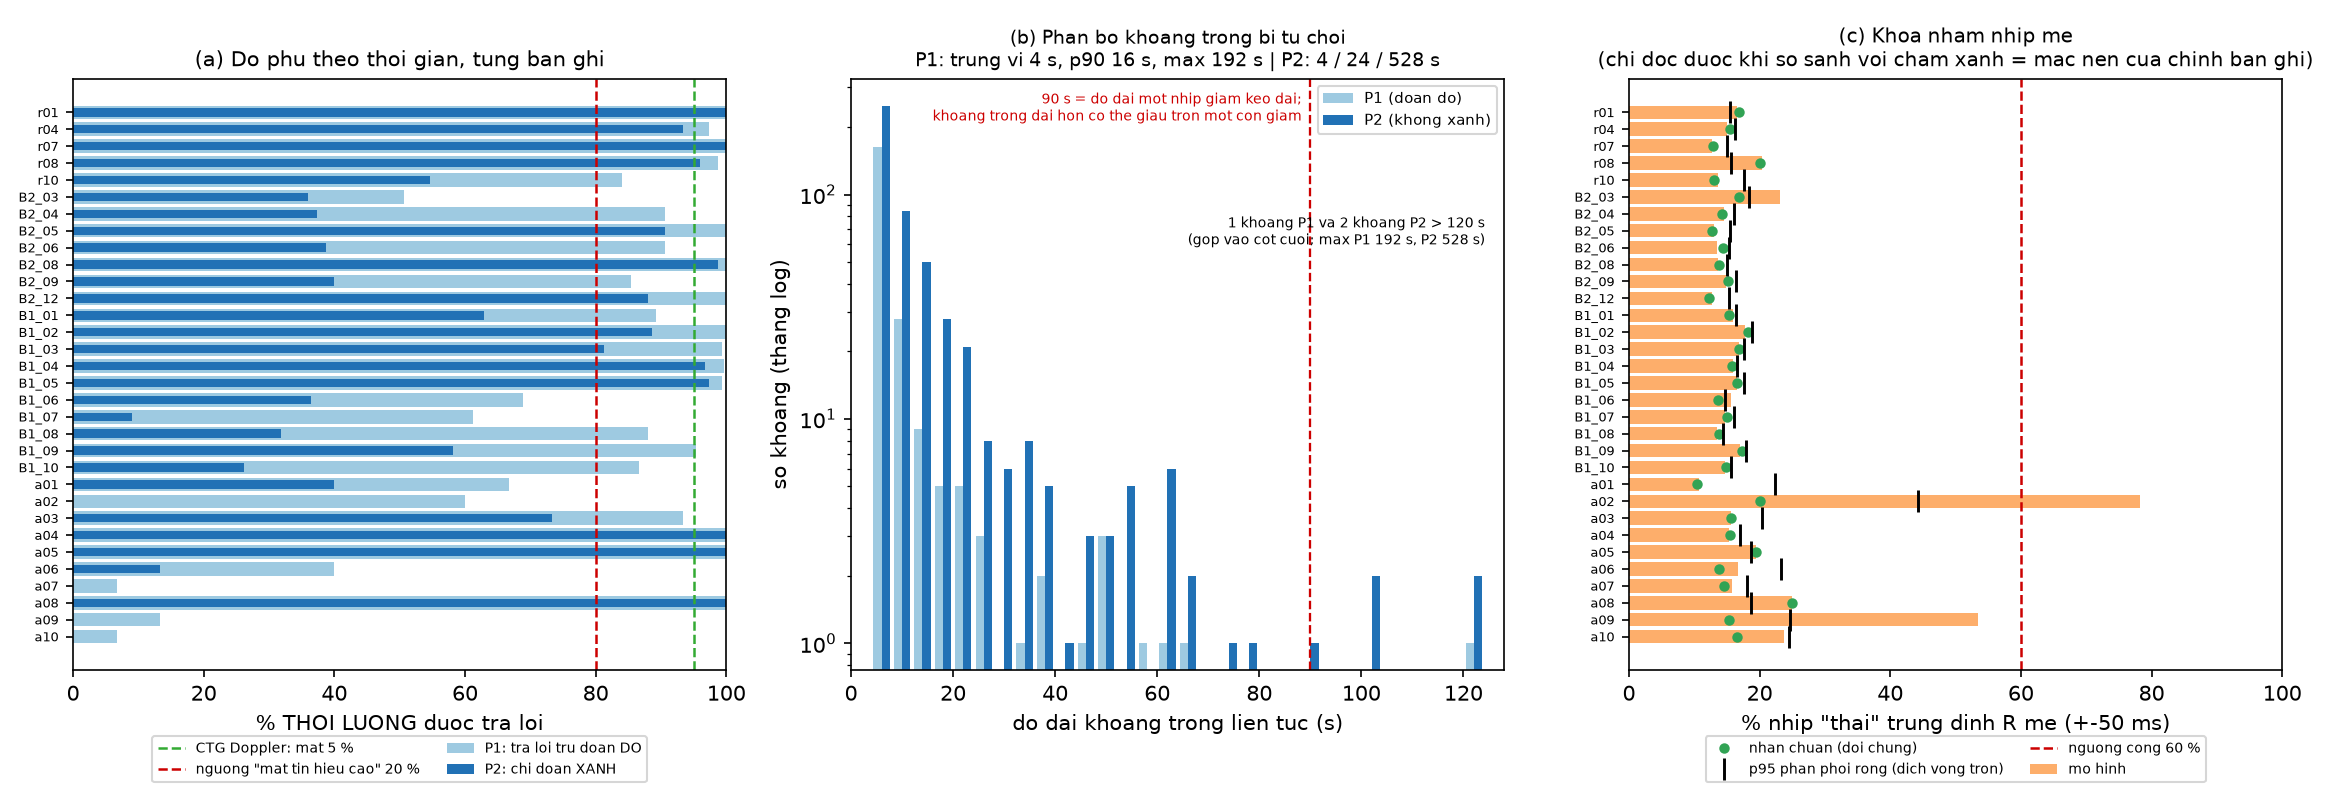
\includegraphics[width=\textwidth]{figs/clinical_coverage_lock.png}
\caption{(a) \% thời lượng trả lời từng bản ghi so với mốc CTG. (b) Phân bố độ dài khoảng trống, thang
log, mốc 90 giây. (c) Khoá nhịp mẹ so với nhãn chuẩn và phân phối rỗng.}
\label{fig:clin_cov}
\end{figure}

\subsection{Chọn kênh sửa được F1, nhưng không sửa được STV}

\begin{table}[H]\centering\small
\caption{Bốn bản ghi CinC 2013 kém nhất: quy tắc PSD mù nhãn so với kênh 0 hậu kiểm. STV tính bằng ms.}
\label{tab:clin_kenh}
\begin{tabular}{@{}C{1.6cm} C{3.6cm} C{3.6cm} C{2.2cm}@{}}
\toprule
\textbf{Bản ghi} & \textbf{PSD: F1 / STV / phủ} & \textbf{Kênh 0: F1 / STV / phủ} & \textbf{STV nhãn} \\
\midrule
a01 & 80,99 / 18,52 / 66,7\,\% & 100,00 / 6,53 / 86,7\,\% & 6,45 \\
a07 & 45,63 / 42,57 / 6,7\,\% & 86,92 / 12,47 / 80,0\,\% & 0,93 \\
a09 & 19,35 / 67,63 / 13,3\,\% & 94,25 / 6,37 / 93,3\,\% & 0,49 \\
a10 & 47,13 / 46,16 / 6,7\,\% & 70,89 / 27,58 / 46,7\,\% & 4,37 \\
\bottomrule
\end{tabular}
\end{table}

Điều đáng chú ý về lâm sàng: \textbf{ngay cả ở kênh 0 với F1 $= 94{,}25$, STV của a09 vẫn là 6,37\,ms so
với nhãn 0,49\,ms --- sai 13 lần}. Vấn đề STV \textbf{không} sửa được bằng cách chọn kênh tốt hơn. Chọn
kênh sửa được F1 và độ phủ; nó không sửa được độ phân giải STV.

\subsection{Những gì mục này KHÔNG chứng minh được}

\begin{enumerate}[leftmargin=1.6em,itemsep=3pt]
\item \textbf{Không có dữ liệu trong vùng ra quyết định.} 22 chủ thể trong miền có STV nhãn 3,49--15,97\,ms;
không ai gần 2,6--3,0\,ms. Không thể ước lượng độ nhạy / độ đặc hiệu của cờ ``STV thấp''.
\item \textbf{22/32 bản ghi ngắn hơn tối thiểu 10 phút của Dawes--Redman} (ADFECGDB và B2 là 5 phút, CinC
là 1 phút). Chỉ 10 bản B1 cho một trị số STV hợp lệ về thời lượng.
\item \textbf{Không có thai dưới 38 tuần trong ADFECGDB}, trong khi giá trị lâm sàng của STV nằm ở tuần
24--37.
\item \textbf{Ngưỡng TRUFFLE 2,6 / 3,0\,ms và các mốc mất tín hiệu CTG đều chưa được nhóm đối chiếu bản
gốc.} Phải kiểm chứng và trích dẫn đúng trước khi đưa vào bài báo.
\item \textbf{STV Dawes--Redman gốc tính trên tín hiệu CTG Doppler lấy mẫu đều}, không phải trên chuỗi RR
từng nhịp. Định nghĩa dùng ở đây là bản thích ứng hợp lý cho fECG nhưng \textbf{không đồng nhất} với
thuật toán gốc.
\item \textbf{Một seed, một fold cho mỗi chủ thể.} B2\_03 --- bản ghi có sai số STV lớn nhất trong miền
($+11{,}99$\,ms) --- cũng chính là bản ghi kém ổn định nhất theo seed ($|$hiệu$|$ 2,81 điểm F1, xem
\S\ref{sec:thongke}). Sai số STV của nó có thể phần lớn là nhiễu huấn luyện.
\item Các hệ số tương quan ở bảng \ref{tab:stv} ($r = 0{,}986$ với $n = 5$) là \textbf{mô tả}, không được
trình bày như bằng chứng thống kê.
\end{enumerate}

\begin{ghichu}[title={Phát biểu cuối cùng về giá trị lâm sàng}]
\hethong{} hiện là \textbf{một bộ đếm nhịp tim thai tốt, không phải một máy đo biến thiên}.
Nhịp tim thai: sai số trung bình dưới 1\,bpm, 95,38\,\% cửa sổ trong $\pm5$\,bpm trên 260 cửa sổ, và
98,66\,\% ngay ở cửa sổ 5 giây trên ADFECGDB --- \textbf{dùng được}.
STV: độ phân giải thiếu 2,5--4,5 lần, sai số một chiều về phía trấn an giả, 3/3 bản ghi tham chiếu thấp
nhất bị bỏ sót --- \textbf{chưa dùng được, và nhóm nói thẳng điều đó thay vì im lặng}.
Độ phủ: đạt chuẩn CTG trên ADFECGDB, chưa đạt trên Silesia, hỏng trên CinC --- và khoảng trống 192 giây
là con số phải sửa trước khi nói đến thử nghiệm lâm sàng.
\end{ghichu}
